\PassOptionsToPackage{unicode=true}{hyperref} % options for packages loaded elsewhere
\PassOptionsToPackage{hyphens}{url}
%
\documentclass[]{article}
\usepackage{lmodern}
\usepackage{amssymb,amsmath}
\usepackage{ifxetex,ifluatex}
\usepackage{fixltx2e} % provides \textsubscript
\ifnum 0\ifxetex 1\fi\ifluatex 1\fi=0 % if pdftex
  \usepackage[T1]{fontenc}
  \usepackage[utf8]{inputenc}
  \usepackage{textcomp} % provides euro and other symbols
\else % if luatex or xelatex
  \usepackage{unicode-math}
  \defaultfontfeatures{Ligatures=TeX,Scale=MatchLowercase}
\fi
% use upquote if available, for straight quotes in verbatim environments
\IfFileExists{upquote.sty}{\usepackage{upquote}}{}
% use microtype if available
\IfFileExists{microtype.sty}{%
\usepackage[]{microtype}
\UseMicrotypeSet[protrusion]{basicmath} % disable protrusion for tt fonts
}{}
\IfFileExists{parskip.sty}{%
\usepackage{parskip}
}{% else
\setlength{\parindent}{0pt}
\setlength{\parskip}{6pt plus 2pt minus 1pt}
}
\usepackage{hyperref}
\hypersetup{
            pdftitle={Final report draft},
            pdfauthor={Rachel Han \& Marion Nyberg},
            pdfborder={0 0 0},
            breaklinks=true}
\urlstyle{same}  % don't use monospace font for urls
\usepackage[margin=1in]{geometry}
\usepackage{color}
\usepackage{fancyvrb}
\newcommand{\VerbBar}{|}
\newcommand{\VERB}{\Verb[commandchars=\\\{\}]}
\DefineVerbatimEnvironment{Highlighting}{Verbatim}{commandchars=\\\{\}}
% Add ',fontsize=\small' for more characters per line
\usepackage{framed}
\definecolor{shadecolor}{RGB}{248,248,248}
\newenvironment{Shaded}{\begin{snugshade}}{\end{snugshade}}
\newcommand{\AlertTok}[1]{\textcolor[rgb]{0.94,0.16,0.16}{#1}}
\newcommand{\AnnotationTok}[1]{\textcolor[rgb]{0.56,0.35,0.01}{\textbf{\textit{#1}}}}
\newcommand{\AttributeTok}[1]{\textcolor[rgb]{0.77,0.63,0.00}{#1}}
\newcommand{\BaseNTok}[1]{\textcolor[rgb]{0.00,0.00,0.81}{#1}}
\newcommand{\BuiltInTok}[1]{#1}
\newcommand{\CharTok}[1]{\textcolor[rgb]{0.31,0.60,0.02}{#1}}
\newcommand{\CommentTok}[1]{\textcolor[rgb]{0.56,0.35,0.01}{\textit{#1}}}
\newcommand{\CommentVarTok}[1]{\textcolor[rgb]{0.56,0.35,0.01}{\textbf{\textit{#1}}}}
\newcommand{\ConstantTok}[1]{\textcolor[rgb]{0.00,0.00,0.00}{#1}}
\newcommand{\ControlFlowTok}[1]{\textcolor[rgb]{0.13,0.29,0.53}{\textbf{#1}}}
\newcommand{\DataTypeTok}[1]{\textcolor[rgb]{0.13,0.29,0.53}{#1}}
\newcommand{\DecValTok}[1]{\textcolor[rgb]{0.00,0.00,0.81}{#1}}
\newcommand{\DocumentationTok}[1]{\textcolor[rgb]{0.56,0.35,0.01}{\textbf{\textit{#1}}}}
\newcommand{\ErrorTok}[1]{\textcolor[rgb]{0.64,0.00,0.00}{\textbf{#1}}}
\newcommand{\ExtensionTok}[1]{#1}
\newcommand{\FloatTok}[1]{\textcolor[rgb]{0.00,0.00,0.81}{#1}}
\newcommand{\FunctionTok}[1]{\textcolor[rgb]{0.00,0.00,0.00}{#1}}
\newcommand{\ImportTok}[1]{#1}
\newcommand{\InformationTok}[1]{\textcolor[rgb]{0.56,0.35,0.01}{\textbf{\textit{#1}}}}
\newcommand{\KeywordTok}[1]{\textcolor[rgb]{0.13,0.29,0.53}{\textbf{#1}}}
\newcommand{\NormalTok}[1]{#1}
\newcommand{\OperatorTok}[1]{\textcolor[rgb]{0.81,0.36,0.00}{\textbf{#1}}}
\newcommand{\OtherTok}[1]{\textcolor[rgb]{0.56,0.35,0.01}{#1}}
\newcommand{\PreprocessorTok}[1]{\textcolor[rgb]{0.56,0.35,0.01}{\textit{#1}}}
\newcommand{\RegionMarkerTok}[1]{#1}
\newcommand{\SpecialCharTok}[1]{\textcolor[rgb]{0.00,0.00,0.00}{#1}}
\newcommand{\SpecialStringTok}[1]{\textcolor[rgb]{0.31,0.60,0.02}{#1}}
\newcommand{\StringTok}[1]{\textcolor[rgb]{0.31,0.60,0.02}{#1}}
\newcommand{\VariableTok}[1]{\textcolor[rgb]{0.00,0.00,0.00}{#1}}
\newcommand{\VerbatimStringTok}[1]{\textcolor[rgb]{0.31,0.60,0.02}{#1}}
\newcommand{\WarningTok}[1]{\textcolor[rgb]{0.56,0.35,0.01}{\textbf{\textit{#1}}}}
\usepackage{graphicx,grffile}
\makeatletter
\def\maxwidth{\ifdim\Gin@nat@width>\linewidth\linewidth\else\Gin@nat@width\fi}
\def\maxheight{\ifdim\Gin@nat@height>\textheight\textheight\else\Gin@nat@height\fi}
\makeatother
% Scale images if necessary, so that they will not overflow the page
% margins by default, and it is still possible to overwrite the defaults
% using explicit options in \includegraphics[width, height, ...]{}
\setkeys{Gin}{width=\maxwidth,height=\maxheight,keepaspectratio}
\setlength{\emergencystretch}{3em}  % prevent overfull lines
\providecommand{\tightlist}{%
  \setlength{\itemsep}{0pt}\setlength{\parskip}{0pt}}
\setcounter{secnumdepth}{0}
% Redefines (sub)paragraphs to behave more like sections
\ifx\paragraph\undefined\else
\let\oldparagraph\paragraph
\renewcommand{\paragraph}[1]{\oldparagraph{#1}\mbox{}}
\fi
\ifx\subparagraph\undefined\else
\let\oldsubparagraph\subparagraph
\renewcommand{\subparagraph}[1]{\oldsubparagraph{#1}\mbox{}}
\fi

% set default figure placement to htbp
\makeatletter
\def\fps@figure{htbp}
\makeatother


\title{Final report draft}
\author{Rachel Han \& Marion Nyberg}
\date{07/03/2020}

\begin{document}
\maketitle

{
\setcounter{tocdepth}{2}
\tableofcontents
}
\hypertarget{introduction}{%
\section{Introduction}\label{introduction}}

This report investigates `Trending YouTube Video Statistics', which was
has records from 2008 and was last updated on 2019-06-02. The primary
aim of the dataset is for use in determining the year's top trending
Youtube videos. Whilst it includes data specific to 10 different
countries, we have chosen to explore the dataset for Canada only.

The dataset contains rows of trending videos which include features like
category, trending date, tags, number of views, likes, dislikes, shares
and descriptions of videos. Previous research has found that despite the
large number of channels on Youtube, on average 85\% of all views go to
just 3\% of channels (Bärtl 2018). We will explore this dataset further
by investigating \textbf{the relationship between video category, number
of views it recieves, likes/dislikes and comment count?} Specificially,
we aim to investigate \textbf{whether the number of views on Youtube
videos correlate with the number of likes or dislikes on a video.}

\hypertarget{about-data}{%
\section{About data}\label{about-data}}

Below are the number of rows and columns for the dataset.

\begin{Shaded}
\begin{Highlighting}[]
\KeywordTok{nrow}\NormalTok{(CAN) }
\end{Highlighting}
\end{Shaded}

\begin{verbatim}
## [1] 40881
\end{verbatim}

\begin{Shaded}
\begin{Highlighting}[]
\KeywordTok{ncol}\NormalTok{(CAN)}
\end{Highlighting}
\end{Shaded}

\begin{verbatim}
## [1] 16
\end{verbatim}

The following are data types of the columns in the dataset.

\begin{Shaded}
\begin{Highlighting}[]
\NormalTok{features <-}\StringTok{ }\NormalTok{CAN }\OperatorTok\StringTok{ }\KeywordTok{colnames}\NormalTok{() }\OperatorTok\StringTok{ }\KeywordTok{tibble}\NormalTok{()}
\NormalTok{types <-}\StringTok{ }\NormalTok{CAN }\OperatorTok\StringTok{ }\KeywordTok{sapply}\NormalTok{(class) }\OperatorTok\StringTok{ }\KeywordTok{tibble}\NormalTok{()}
\NormalTok{feature_type <-}\StringTok{ }\KeywordTok{cbind}\NormalTok{(features,types)}
\KeywordTok{colnames}\NormalTok{(feature_type)<-}\KeywordTok{c}\NormalTok{(}\StringTok{"Features"}\NormalTok{,}\StringTok{"Type"}\NormalTok{)}
\KeywordTok{kable}\NormalTok{(feature_type) }\OperatorTok\StringTok{  }\NormalTok{kableExtra}\OperatorTok{::}\KeywordTok{kable_styling}\NormalTok{(}\DataTypeTok{full_width =}\NormalTok{ F)}
\end{Highlighting}
\end{Shaded}

Features

Type

video\_id

character

trending\_date

Date

title

character

channel\_title

character

category\_id

numeric

publish\_time

logical

tags

character

views

numeric

likes

numeric

dislikes

numeric

comment\_count

numeric

thumbnail\_link

character

comments\_disabled

logical

ratings\_disabled

logical

video\_error\_or\_removed

logical

description

character

\hypertarget{eda}{%
\section{EDA}\label{eda}}

\hypertarget{trend-in-views-and-likes}{%
\subsection{Trend in views and likes}\label{trend-in-views-and-likes}}

Below we plot number of likes as a function of views.

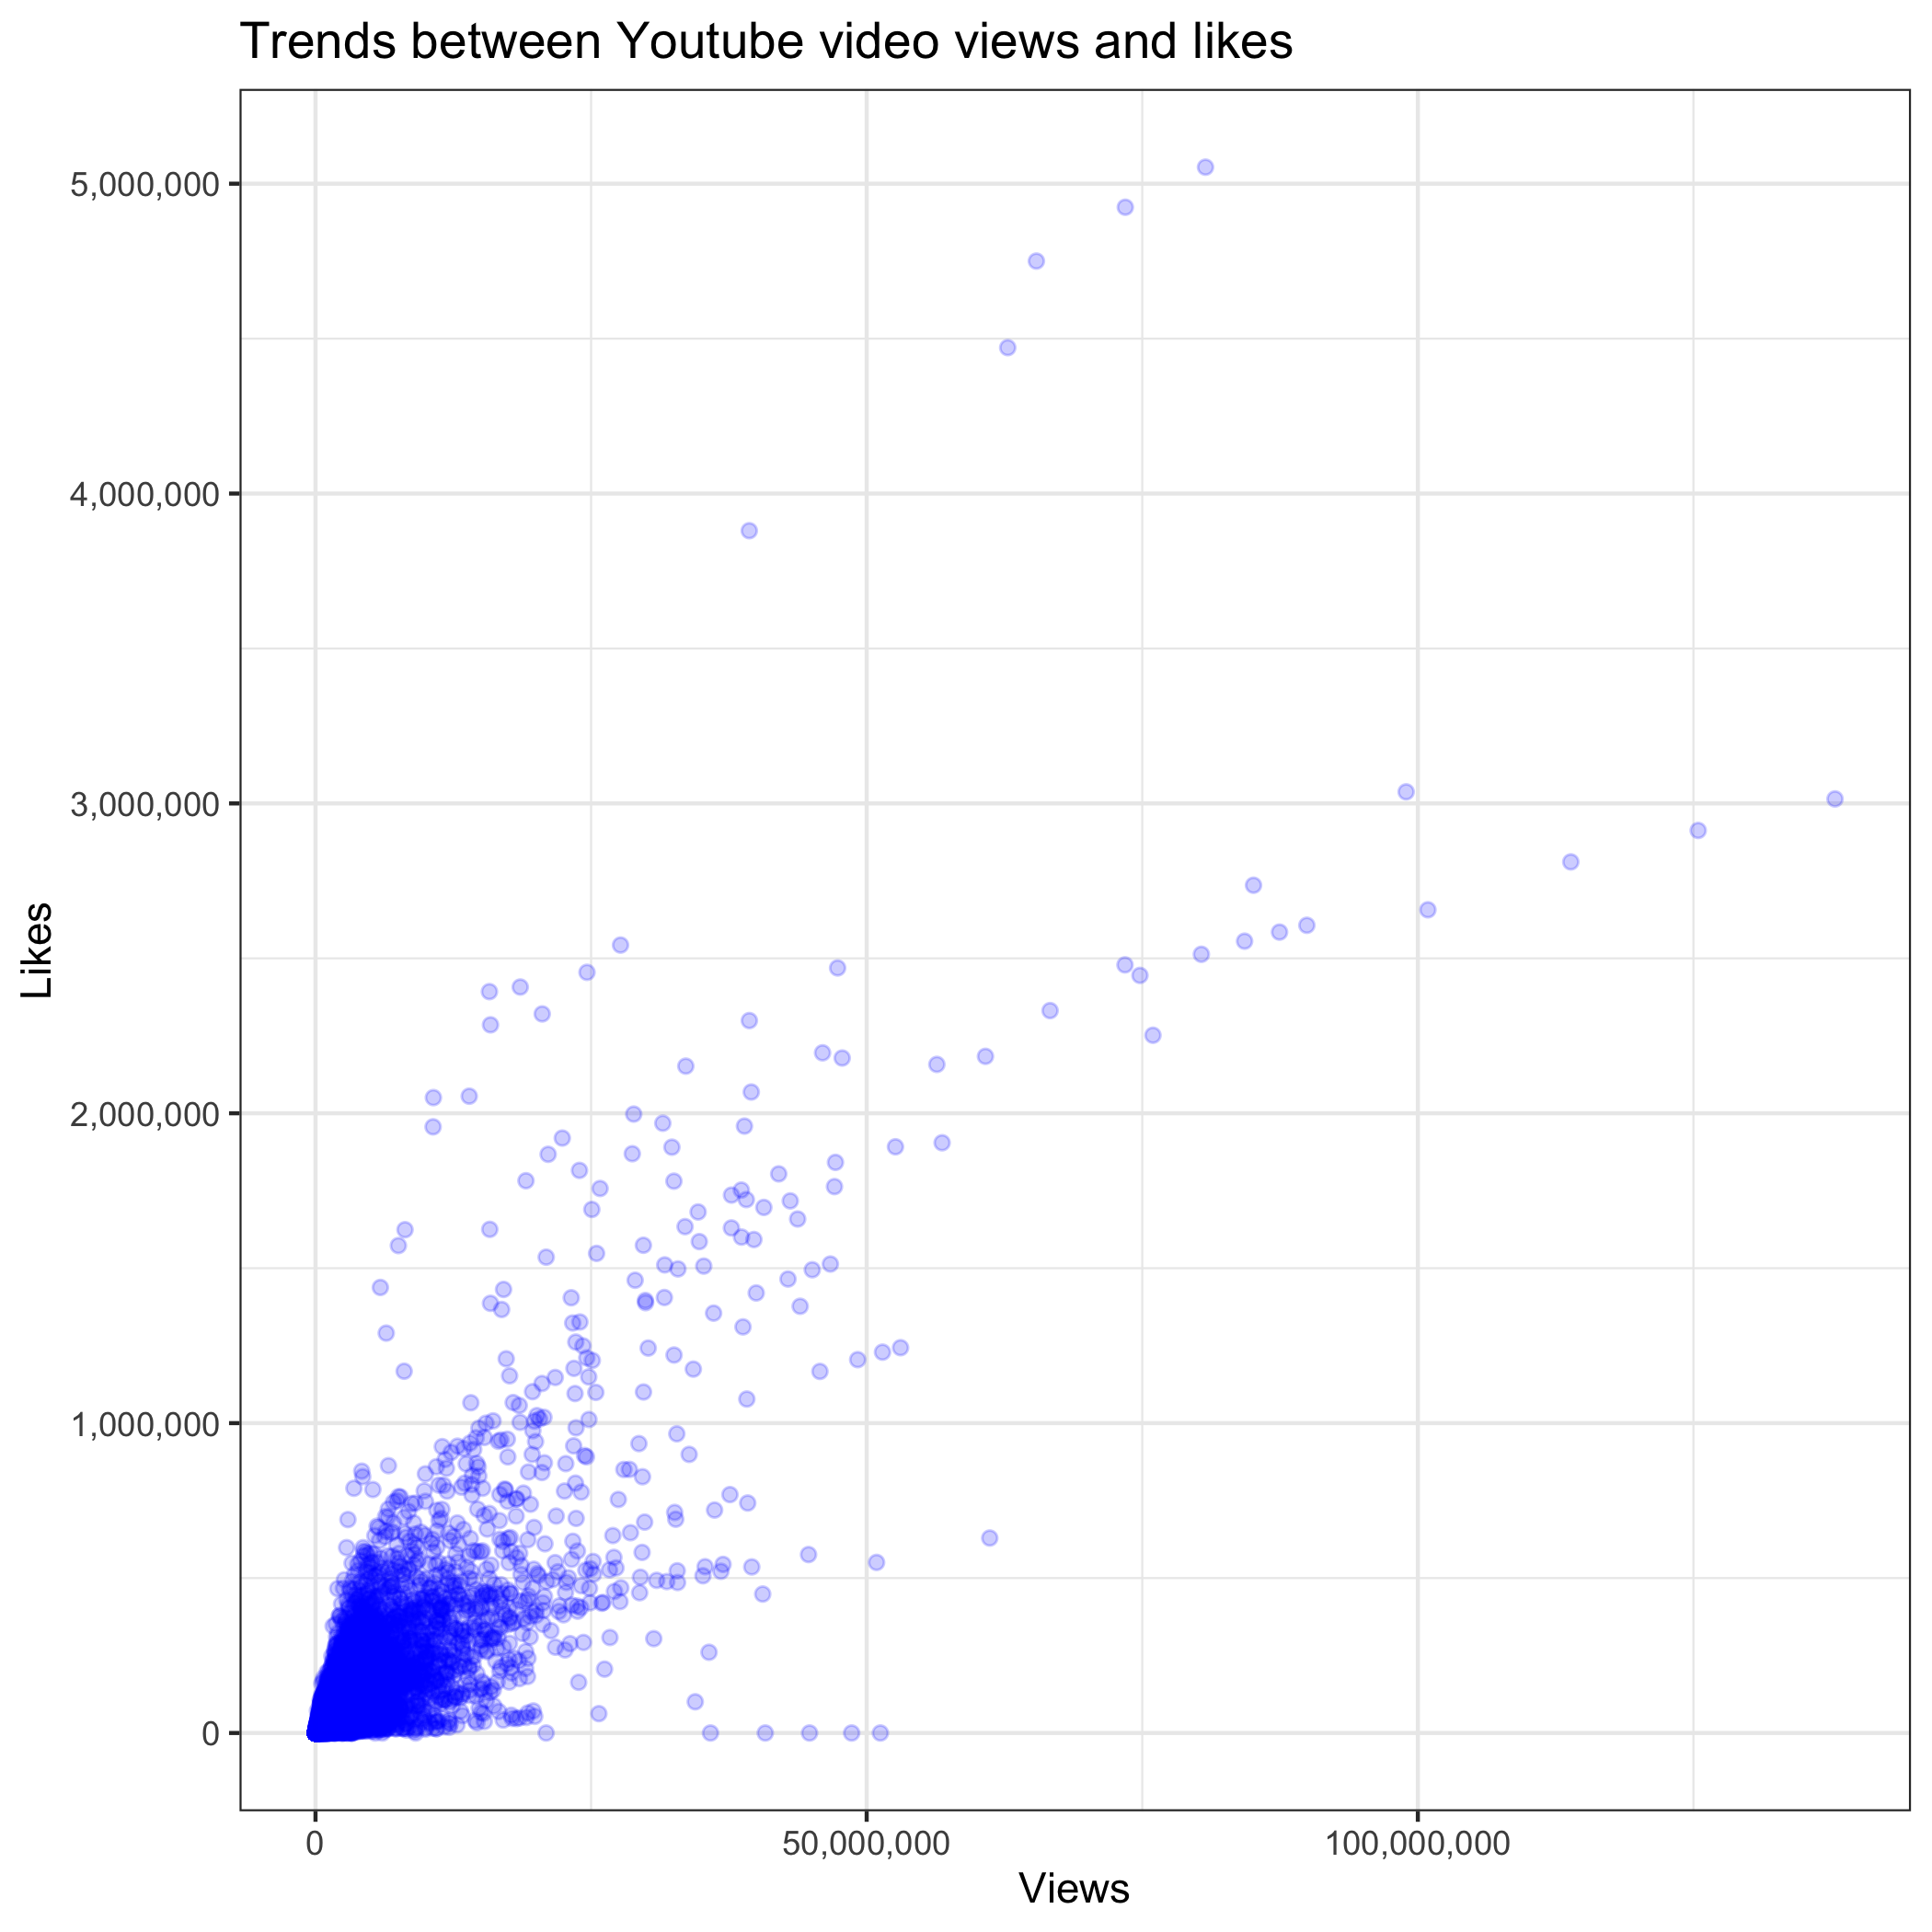
\includegraphics{../images/views_likes.png}

We see that in general the number of likes increase as we have more
views. The points are concentrated at the bottom left corner (there are
more videos with number of views less than 50 million, and likes less
than 1 million).

\hypertarget{number-of-videos-in-each-category.}{%
\subsection{Number of videos in each
category.}\label{number-of-videos-in-each-category.}}

We explore how many videos are in each category.

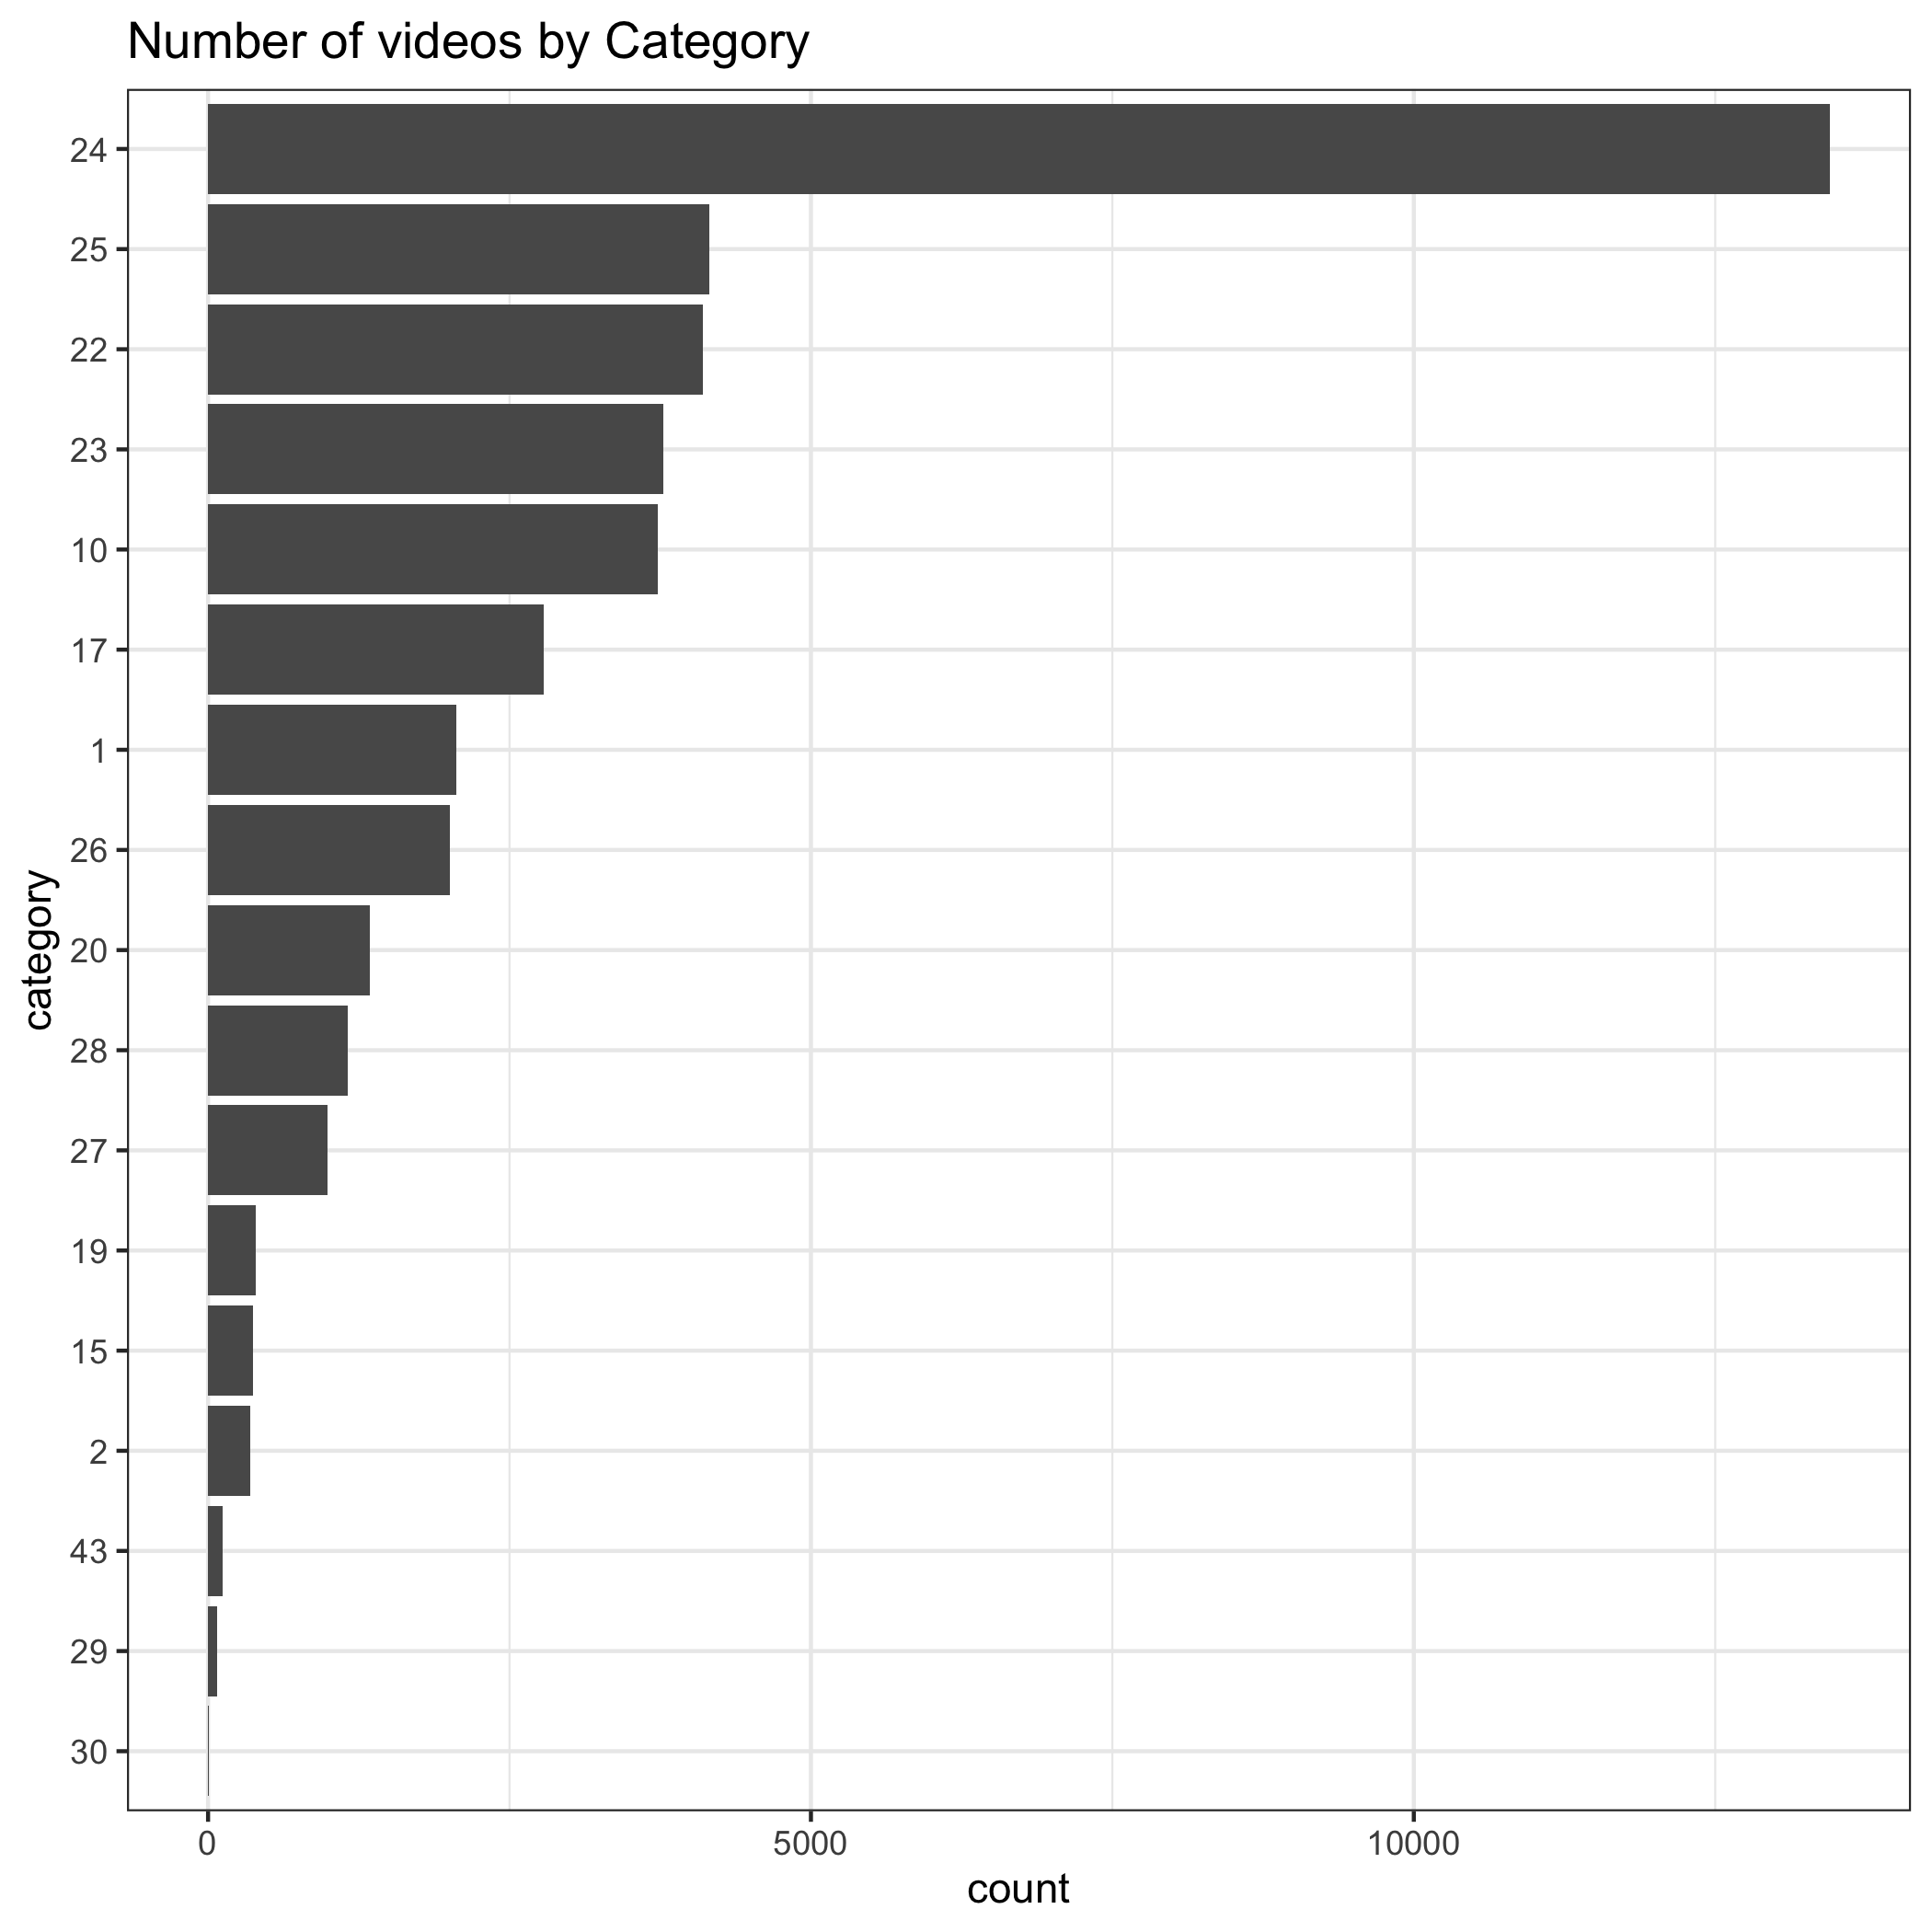
\includegraphics{../images/num_vids_category.png} The category
corresponding to its ID can be found
\href{https://developers.google.com/youtube/v3/docs/videoCategories/list}{here}.

Top 5 Categories are:

\begin{itemize}
\tightlist
\item
  Category 24: Entertainment
\item
  Category 25: News and Politics
\item
  Category 22: People and Blogs
\item
  Category 23: Comedy
\item
  Category 10: Music
\end{itemize}

Bottom 5 Categories are:

\begin{itemize}
\tightlist
\item
  Category 30: Movies
\item
  Category 29: Nonprofits \& Activism
\item
  Category 43: Shows
\item
  Category 2: Autos and Vehicles
\item
  Category 15: Pets and Animals
\end{itemize}

\hypertarget{correlation-plot}{%
\subsection{Correlation plot}\label{correlation-plot}}

Next, we explore correlation between numerical columns.

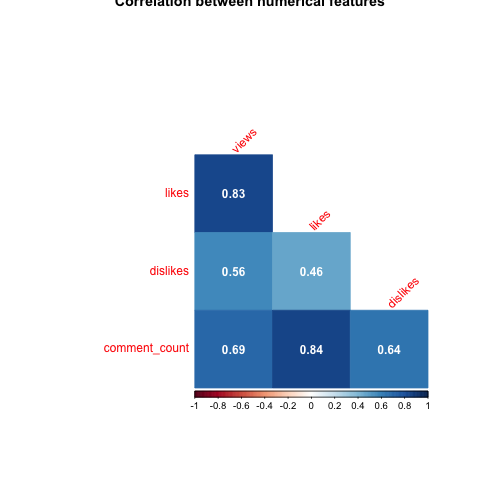
\includegraphics{../images/corr_plot.png}

We note the highest correlation between the number of likes and number
of comments, and the lowest correlation beetween number of views and
number of dislikes.

\hypertarget{analysis-methods}{%
\section{Analysis methods}\label{analysis-methods}}

We explore the relationship between the number of views and number of
likes and dislikes. We aim to build a regression model of \texttt{views}
as a function of \texttt{likes} and \texttt{dislikes}. It is reasonable
to assume that the dependent variable is \texttt{views} and the
explanatory variables are \texttt{likes} and \texttt{dislikes}. One
could switch these response and explanatory variables depending on their
interpretation.

We use linear regression to fit the model.

\begin{Shaded}
\begin{Highlighting}[]
\NormalTok{fit.lm <-}\StringTok{ }\KeywordTok{readRDS}\NormalTok{(}\DataTypeTok{file=}\StringTok{"../rds/lm.rds"}\NormalTok{)}
\end{Highlighting}
\end{Shaded}

We also use poisson regression method. We choose this method because the
response variable \texttt{views} is actually a count data, and may
follow Poisson distribution.

\begin{Shaded}
\begin{Highlighting}[]
\NormalTok{fit.glm <-}\KeywordTok{readRDS}\NormalTok{(}\DataTypeTok{file=}\StringTok{"../rds/glm.rds"}\NormalTok{)}
\end{Highlighting}
\end{Shaded}

\hypertarget{results}{%
\section{Results}\label{results}}

We check the summary of the linear model. \texttt{r.squared} denotes the
goodness of fit of the data, measured by the ratio between the variance
of the fitted values and variance of the actual values (response
variable = \texttt{views}). We see that it is close to 0, which means
the data is poorly fitted.

\begin{Shaded}
\begin{Highlighting}[]
\KeywordTok{glance}\NormalTok{(fit.lm)}
\end{Highlighting}
\end{Shaded}

\begin{verbatim}
## # A tibble: 1 x 11
##   r.squared adj.r.squared  sigma statistic p.value    df  logLik    AIC    BIC
##       <dbl>         <dbl>  <dbl>     <dbl>   <dbl> <int>   <dbl>  <dbl>  <dbl>
## 1     0.726         0.726 1.77e6    54283.       0     3 -6.46e5 1.29e6 1.29e6
## # ... with 2 more variables: deviance <dbl>, df.residual <int>
\end{verbatim}

Below is the diagnostic plot of the linear model, showing residual
vs.~fitted values. We see that the fitted values are aggressively
clustered at lower end with low residual. We have a number of outliers.

\begin{Shaded}
\begin{Highlighting}[]
\KeywordTok{plot}\NormalTok{(fit.lm,}\DataTypeTok{which=}\DecValTok{1}\NormalTok{)}
\end{Highlighting}
\end{Shaded}

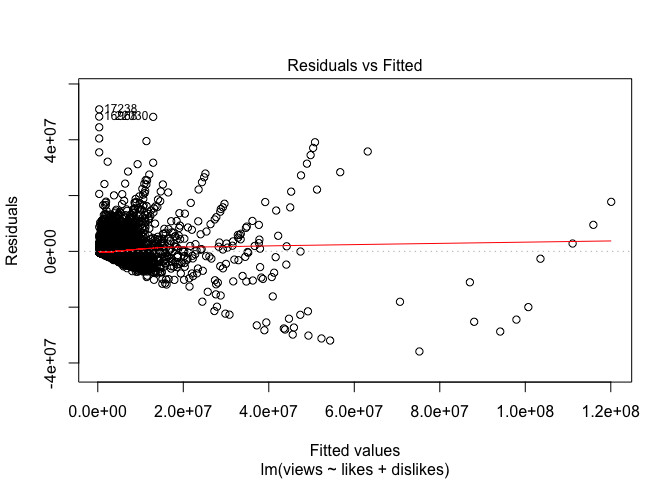
\includegraphics{finalreport_files/figure-latex/unnamed-chunk-7-1.pdf}

Here is a plot that performs linear regression on views with one
explanotory variable each, \texttt{likes} and \texttt{dislikes}.
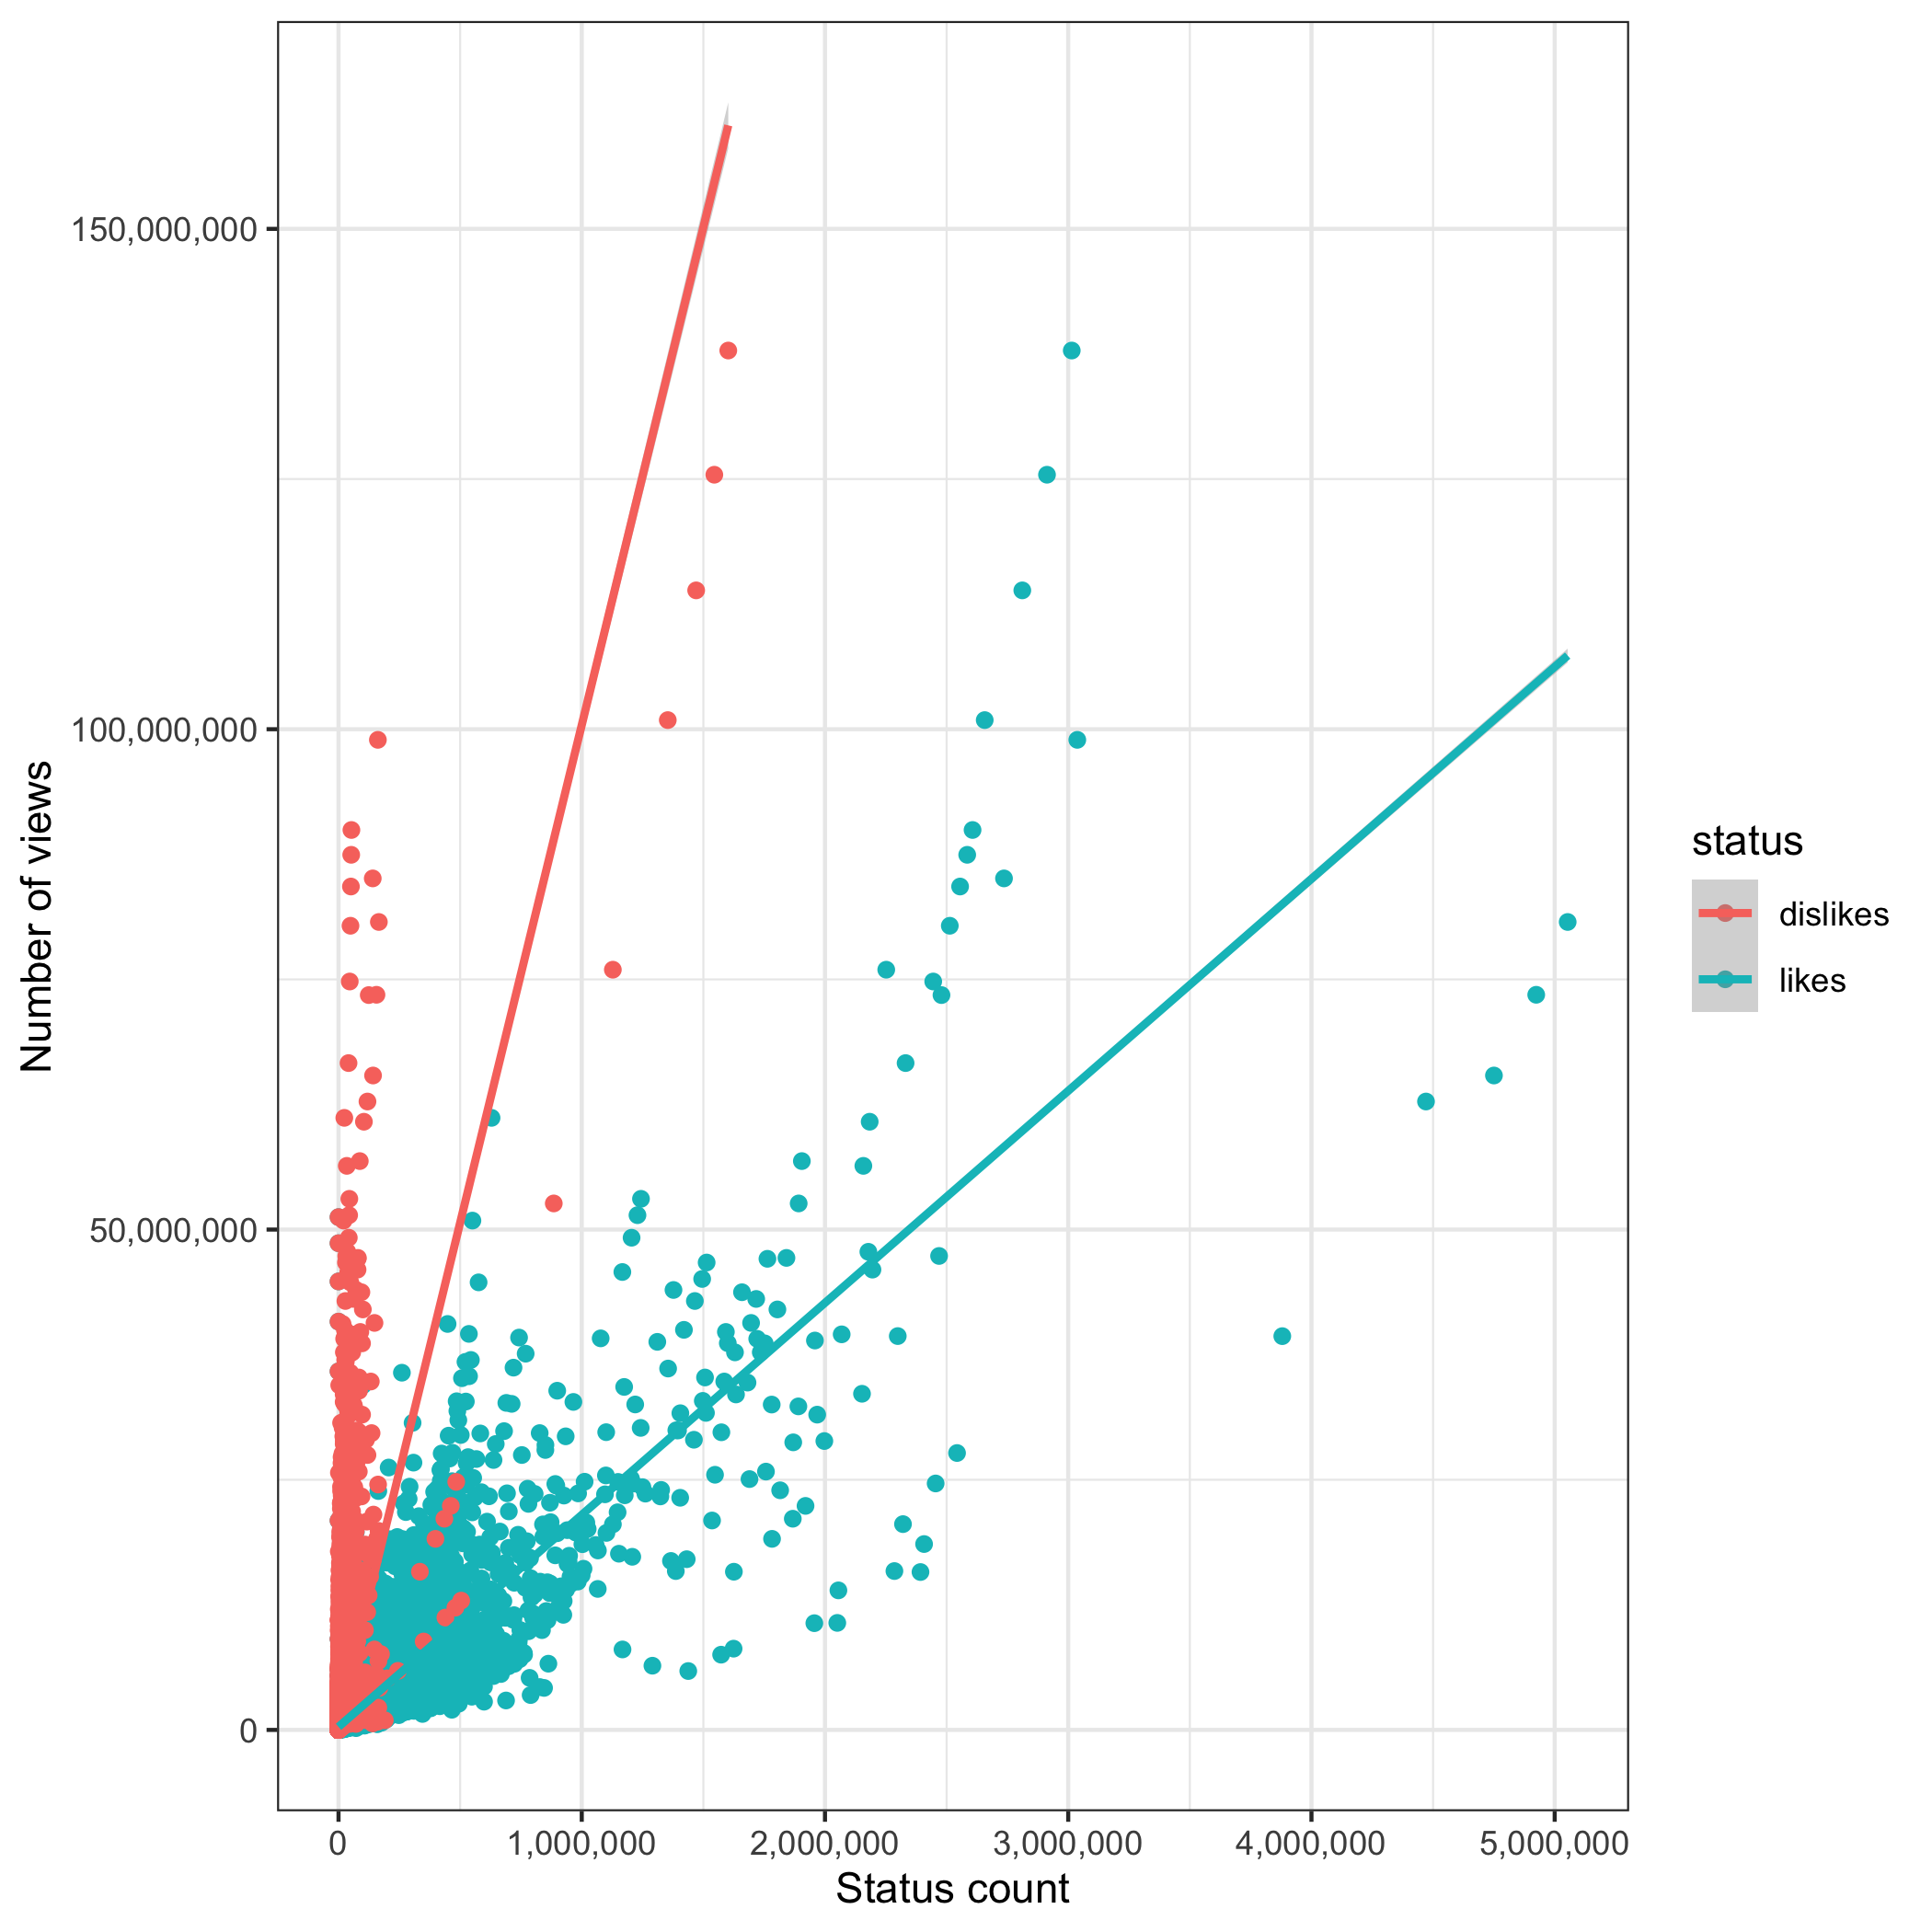
\includegraphics{../images/lm_status_views.png}

Although we see a poor fit, we see that it does capture the trend that
as number of likes or dislikes increase, the views also increase.

Next we present the residuals vs fitted plot from poisson regression. We
see that the residuals do not exceed 1e+7 like in the linear regression,
but we still see skewed distribution of the points. As the value of
fitted values (\texttt{views}) increase, the more deviation we have from
the actual value. This suggests that neither linear or poisson
regression does well in modelling \texttt{views} at higher values.

\begin{Shaded}
\begin{Highlighting}[]
\KeywordTok{plot}\NormalTok{(fit.glm,}\DataTypeTok{which=}\DecValTok{1}\NormalTok{)}
\end{Highlighting}
\end{Shaded}

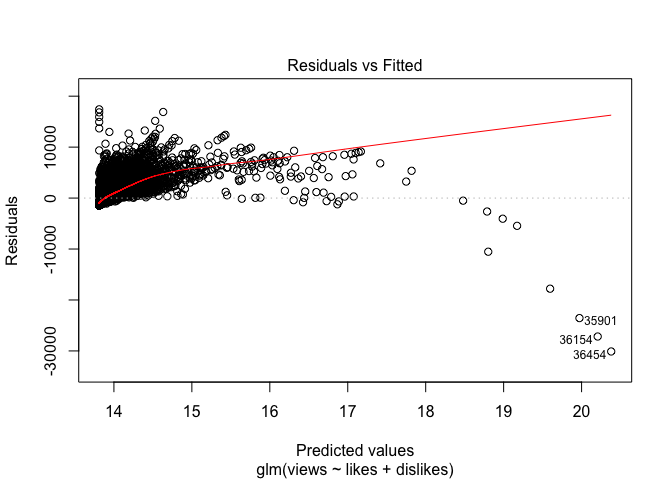
\includegraphics{finalreport_files/figure-latex/unnamed-chunk-8-1.pdf}

Here is a plot that performs poisson regression on views with
\texttt{likes} and \texttt{dislikes}. The model exhibits an exponential
behaviour. It fits reasonably well for the lower values for the response
variable but quickly overshoots.
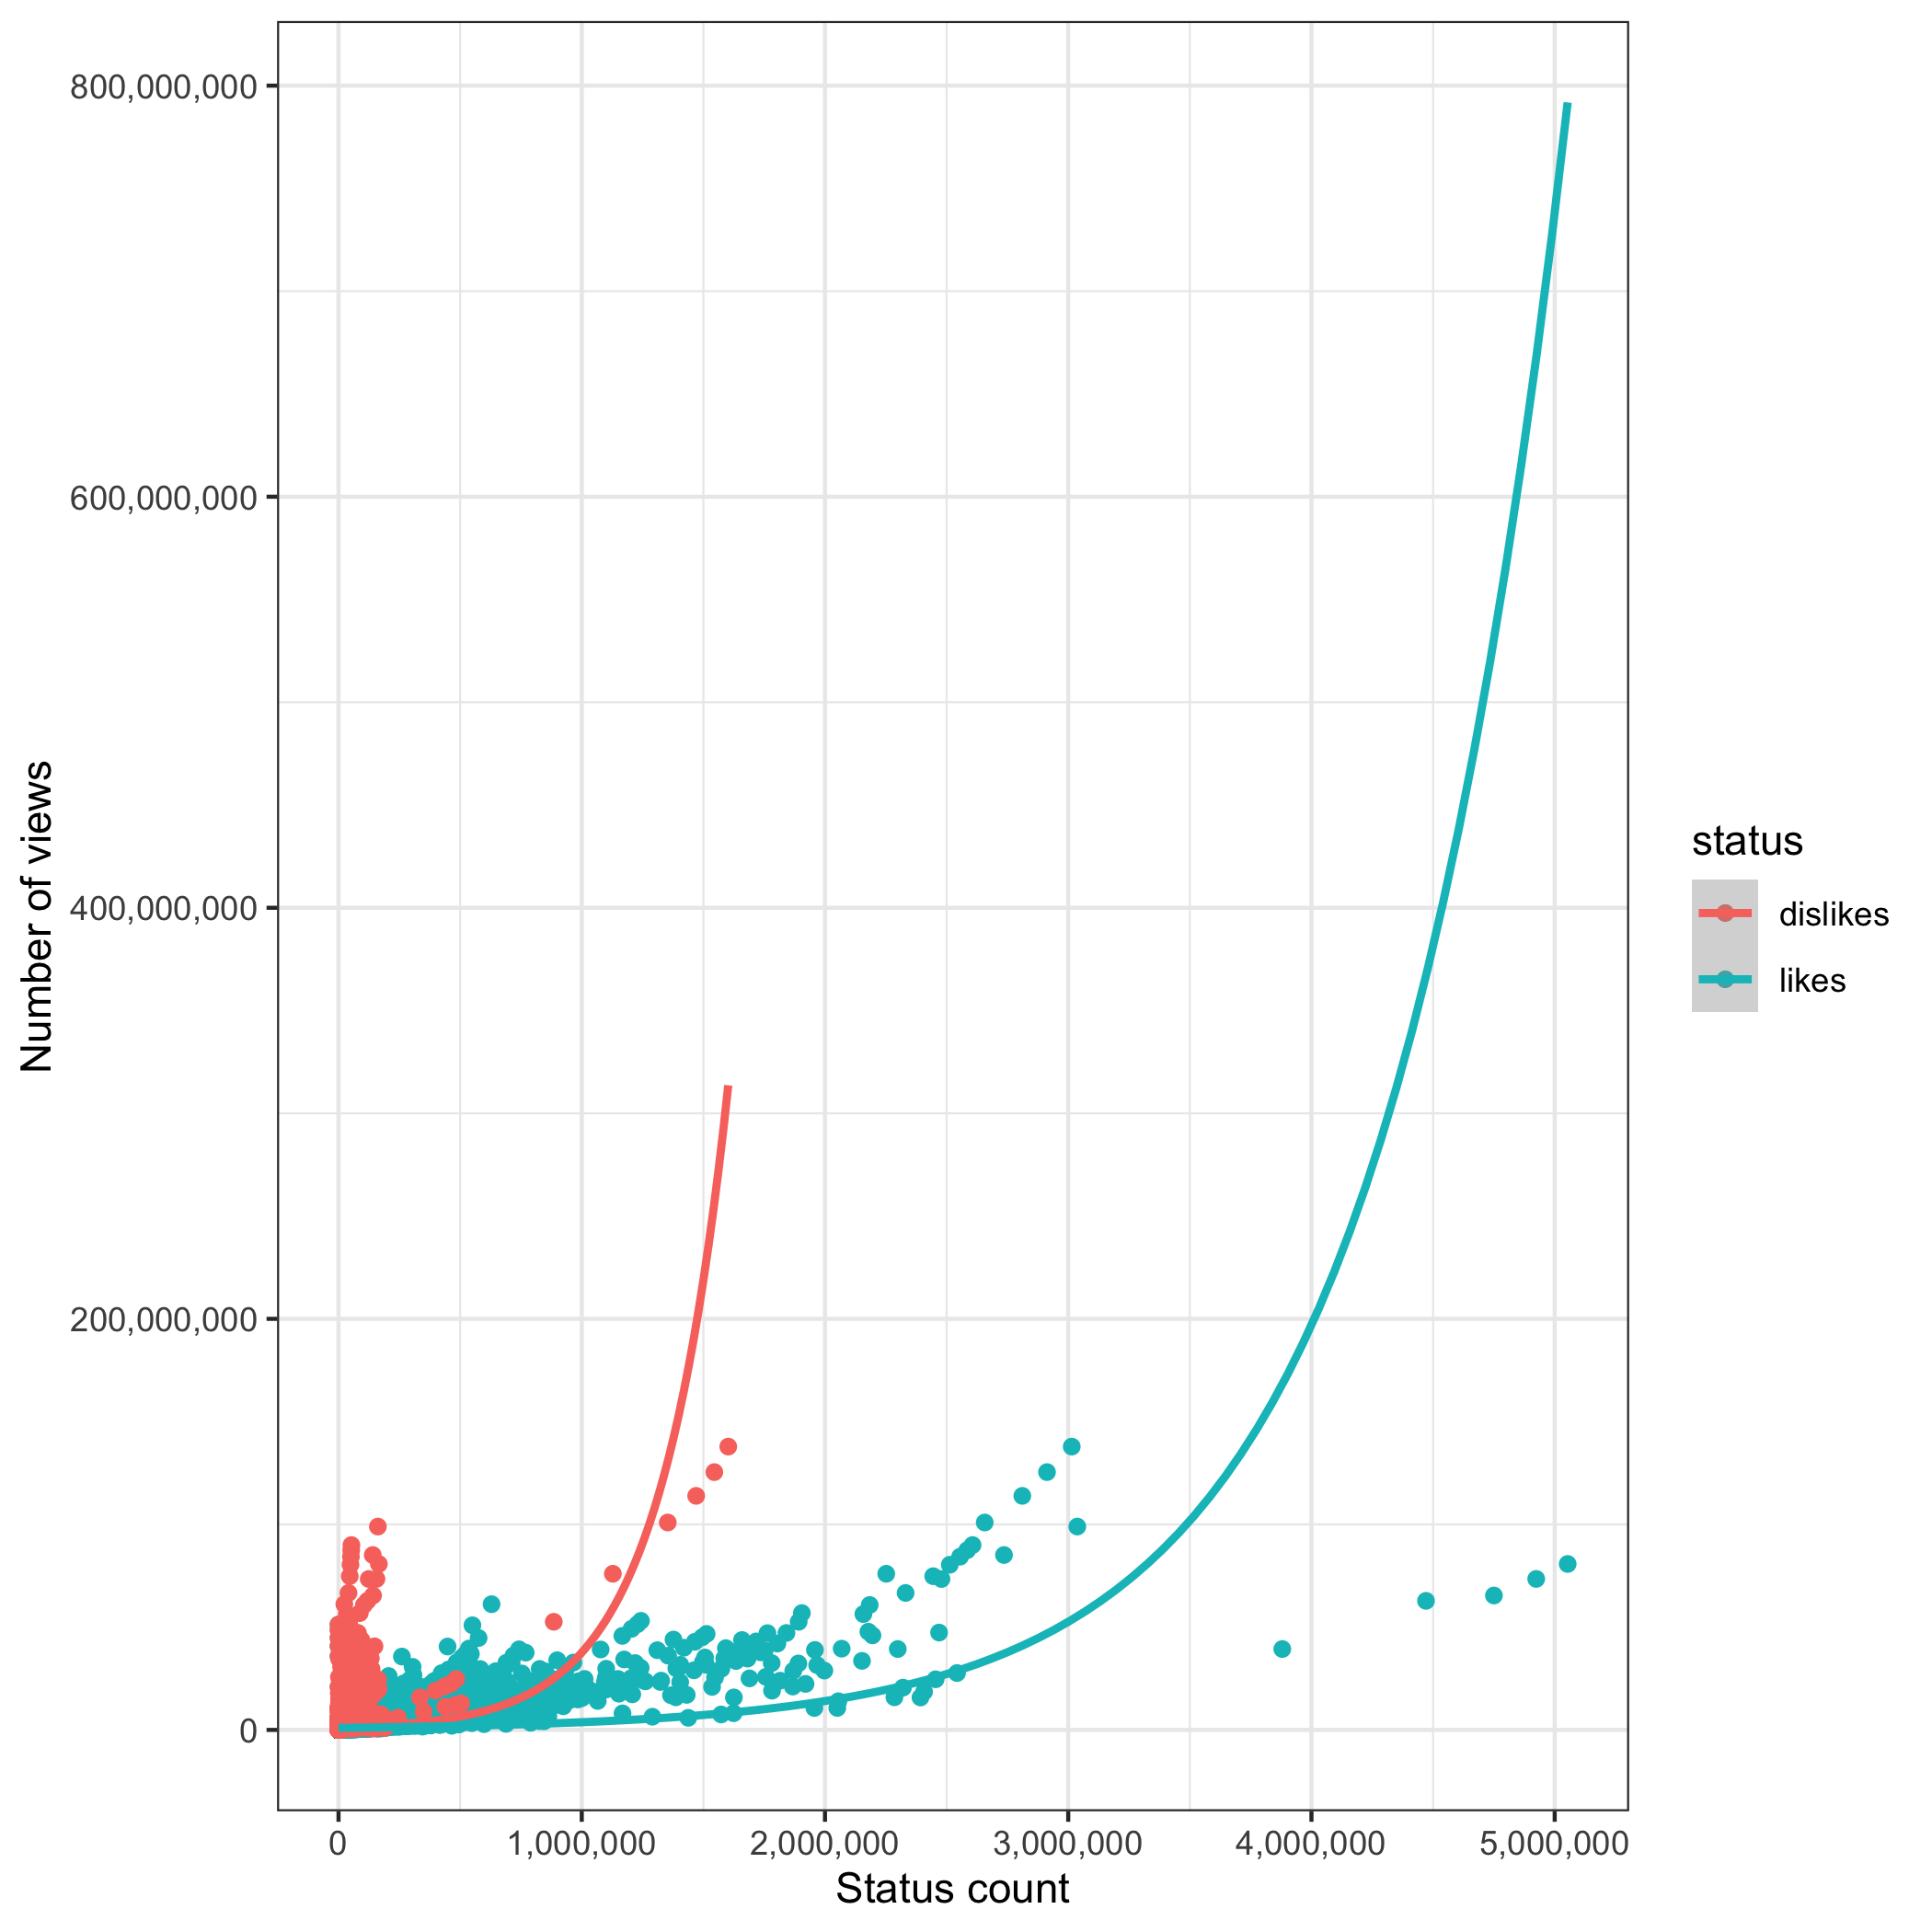
\includegraphics{../images/pois_status_views.png}

We compute the sum of the squared residuals of both models and observe
that poisson regression yields a smaller number. One reason might be
that the sum of the residuals from the outliers in poisson regression
does not outweigh the total sum of residuals in linear regression.

\begin{Shaded}
\begin{Highlighting}[]
\KeywordTok{sum}\NormalTok{(}\KeywordTok{resid}\NormalTok{(fit.lm)}\OperatorTok{^}\DecValTok{2}\NormalTok{)}
\end{Highlighting}
\end{Shaded}

\begin{verbatim}
## [1] 1.285747e+17
\end{verbatim}

\begin{Shaded}
\begin{Highlighting}[]
\KeywordTok{sum}\NormalTok{(}\KeywordTok{resid}\NormalTok{(fit.glm)}\OperatorTok{^}\DecValTok{2}\NormalTok{)}
\end{Highlighting}
\end{Shaded}

\begin{verbatim}
## [1] 78292616784
\end{verbatim}

\hypertarget{discussionconclusion}{%
\section{Discussion/Conclusion}\label{discussionconclusion}}

We have explored the YouTube dataset from Kaggle in this report by a
scatter plot, bar graph and a correlation plot to observe trends in the
data. Then we performed regression analysis on \texttt{views} which we
assumed is a function of \texttt{likes} and \texttt{dislikes}. We
encountered difficulty in fitting the model with both linear and poisson
regression, due to the outliers. One way to deal with this is to create
a weight vector such that the outliers carry little weights. This may be
studied for our future work.

\hypertarget{references}{%
\section{References}\label{references}}

Bärtl, M. (2018). YouTube channels, uploads and views: A statistical
analysis of the past 10 years. Convergence, 24(1), 16--32.
\url{https://doi.org/10.1177/1354856517736979}

\end{document}
